\section{Benchmark NIST-11 "Intersecting Interfaces"}
\label{sec:bench-11}

This is a Poisson's problem with intersecting interfaces,
dividing the plane into four regions.
The solution to this problem contains a severe
singularity that poses a challenge to adaptive methods.
The equation solved is given by

\begin{equation} \label{intersecting}
-\nabla \cdot (a(x,y) \nabla u) = 0
\end{equation}
where the parameter $a$ is piecewise-constant,
$a(x,y) = 161.4476387975881$ in the first and third quadrants,
and $a(x,y) = 1$ in the remaining two quadrants.
The domain of this problem is $\Omega = (-1, 1)^2$, equipped with
Dirichlet boundary conditions given by the exact solution.
The exact solution is
$u(x,y) = r^{a_1} \mu (\theta)$,
where $a_1$ and $\mu (\theta)$ is given in \cite{mitchell-1}.
The right-hand side $f$ is calculated by inserting exact solution into (\ref{intersecting}).
The solution of NIST-11 is shown in Fig. \ref{fig:sln-nist11}.

\begin{figure}[!ht]
\centering
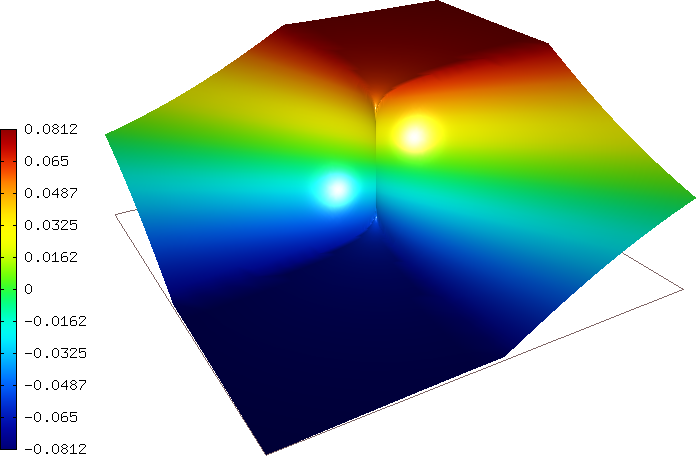
\includegraphics[height=5cm]{nist/nist-11/solution.png}
\caption{The solution to NIST-11 benchmark problem.}
\label{fig:sln-nist11}
\end{figure}

\begin{figure}[!ht]
\centering
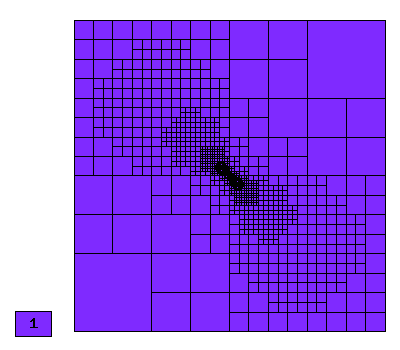
\includegraphics[height=3.7cm]{nist/nist-11/mesh_h1_aniso.png}
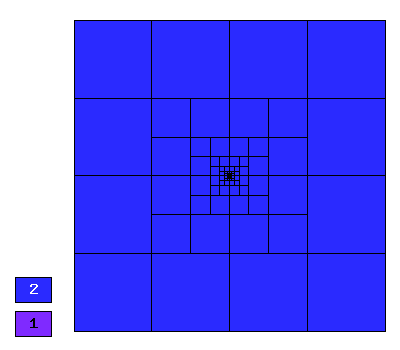
\includegraphics[height=3.7cm]{nist/nist-11/mesh_h2_aniso.png}
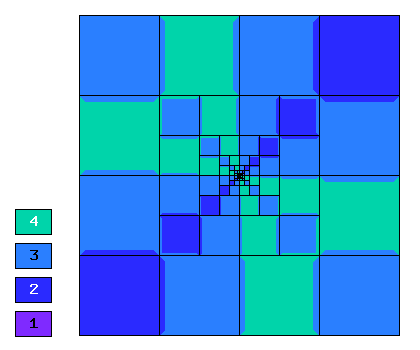
\includegraphics[height=3.7cm]{nist/nist-11/mesh_hp_aniso.png}
\caption{
Final mesh (left) with 46905 DOF and the resulting
relative error estimate in $H^1$-norm of 1.25659 \% for $h$-FEM with linear elements.
Final mesh (middle) with 7777 DOF and the resulting
relative error estimate in $H^1$-norm of 4.73604e-01 \% for $h$-FEM with quadratic elements.
Final mesh (right) with 3459 DOF and the resulting 
relative error estimate in $H^1$-norm of 4.7087e-01 \% for $hp$-FEM with anisotropic refinements.}
\label{fig:nist-11-hp-aniso}
\end{figure}

%\begin{figure}[!ht]
%\centering
%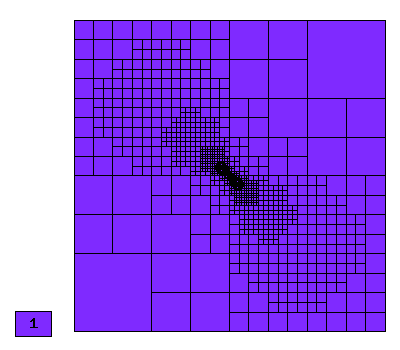
\includegraphics[height=5cm]{nist/nist-11/mesh_h1_aniso.png}\ \
%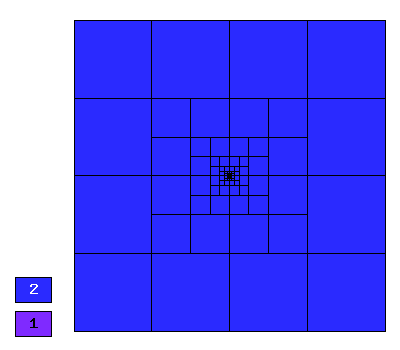
\includegraphics[height=5cm]{nist/nist-11/mesh_h2_aniso.png}
%\caption{Final mesh for $h$-FEM with linear and quadratic elements.}
%\label{fig:nist-11-h-aniso}
%\end{figure}

Figs. \ref{fig:nist-11-conv} compare all
three approaches to automatic adaptivity from the point
of view of DOF and CPU convergence.

\begin{figure}[!ht]
\centering
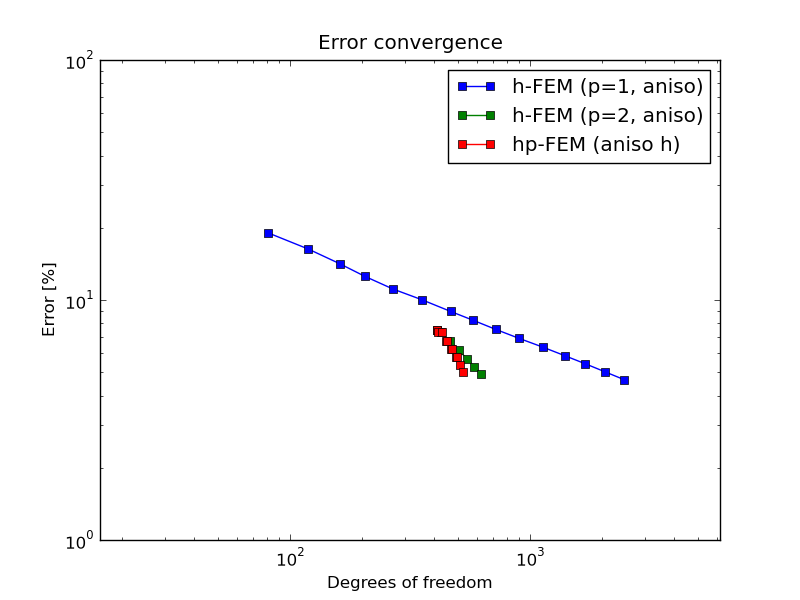
\includegraphics[height=5cm]{nist/nist-11/conv_dof_aniso.png}\ \
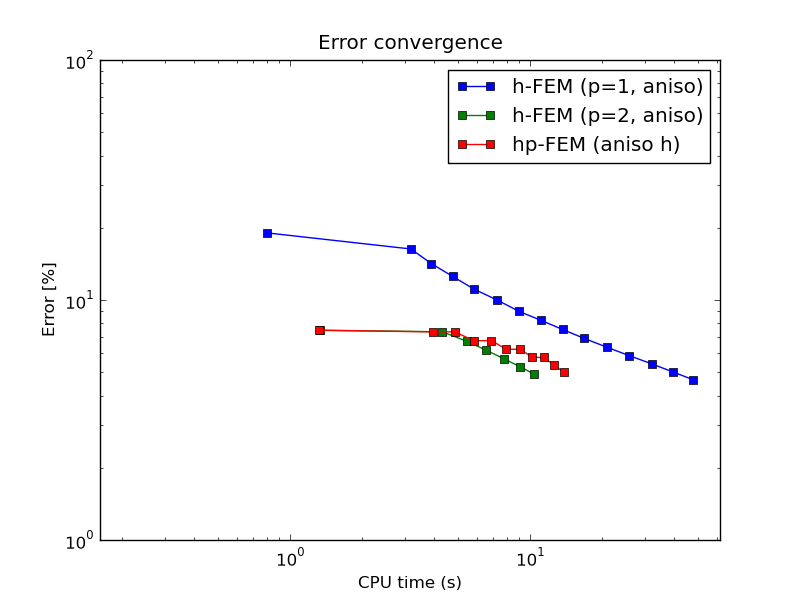
\includegraphics[height=5cm]{nist/nist-11/conv_cpu_aniso.png}
\caption{DOF and CPU time convergence graphs.}
\label{fig:nist-11-conv}
\end{figure}

